\documentclass[aspectratio=169]{beamer}

\usetheme{default}
\useinnertheme{rounded}
\useoutertheme{infolines}
\setbeamertemplate{navigation symbols}{}
\setbeamertemplate{footline}[frame number]

\usepackage[T1]{fontenc}
\usepackage{graphicx}
\usepackage{booktabs}
\usepackage{array}
\usepackage{xcolor}

\graphicspath{{figures/}{./}}

\definecolor{garudadark}{RGB}{52,58,64}
\definecolor{garudamid}{RGB}{108,117,125}
\definecolor{garudalight}{RGB}{233,236,239}
\definecolor{garudaaccent}{RGB}{73,80,87}

\setbeamercolor{normal text}{fg=garudadark,bg=white}
\setbeamercolor{title}{fg=white,bg=garudadark}
\setbeamercolor{frametitle}{fg=white,bg=garudadark}
\setbeamercolor{subtitle}{fg=garudalight}
\setbeamercolor{author}{fg=garudadark}
\setbeamercolor{institute}{fg=garudamid}
\setbeamercolor{date}{fg=garudamid}
\setbeamercolor{structure}{fg=garudaaccent}
\setbeamercolor{palette primary}{fg=white,bg=garudadark}
\setbeamercolor{palette secondary}{fg=white,bg=garudaaccent}
\setbeamercolor{palette tertiary}{fg=white,bg=garudamid}
\setbeamercolor{block title}{fg=white,bg=garudaaccent}
\setbeamercolor{block body}{fg=garudadark,bg=garudalight}
\setbeamercolor{item projected}{fg=white,bg=garudaaccent}
\setbeamercolor{section in toc}{fg=garudadark}

\setbeamerfont{title}{series=\bfseries,size=\LARGE}
\setbeamerfont{frametitle}{series=\bfseries,size=\large}
\setbeamerfont{block title}{series=\bfseries}

\title[Garuda Project Brief]{Garuda: Privacy-First Edge-AI Home Security}
\subtitle{Brief project presentation based on the paper draft}
\author{Gonugondla Veera Manikanta}
\institute{Manipal Institute of Technology}
\date{\today}

\begin{document}

\begin{frame}
  \titlepage
\end{frame}

\begin{frame}{Problem and Goal}
  \begin{itemize}
    \item Cloud cameras are convenient, but they send private footage off-device and usually require subscriptions.
    \item DIY home-security builds keep data local, but many stop at simple motion detection and weak alert pipelines.
    \item Garuda targets the gap: accurate threat detection, local processing, secure access, and practical deployment on low-power hardware.
    \item The paper focuses on a measured system integration result, not a new detection algorithm.
  \end{itemize}
\end{frame}

\begin{frame}{Core Idea}
  \begin{columns}[T]
    \begin{column}{0.54\textwidth}
      \begin{itemize}
        \item All camera inference stays on-device.
        \item Raspberry Pi 5 hosts the services layer.
        \item Hailo-8L NPU handles real-time neural inference.
        \item FastAPI dashboard, remote access, alerts, logging, and voice control run alongside detection.
      \end{itemize}
      \vspace{0.3cm}
      \textbf{Design priority:} privacy first, real-time response, low recurring cost.
    \end{column}
    \begin{column}{0.46\textwidth}
      \centering
      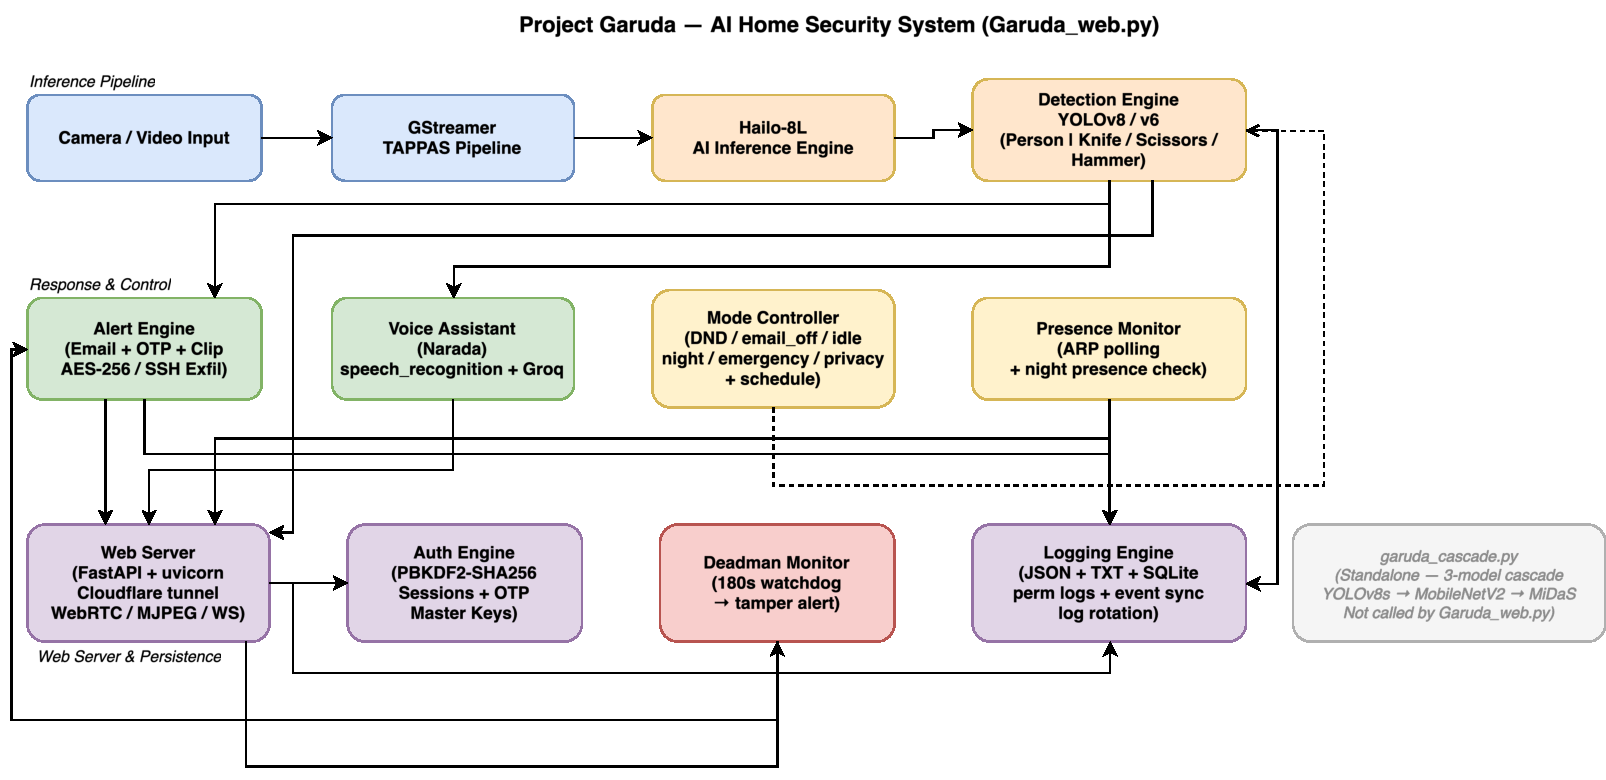
\includegraphics[width=\linewidth,height=0.68\textheight,keepaspectratio]{garuda_block_diagram.drawio-3.pdf}
    \end{column}
  \end{columns}
\end{frame}

\begin{frame}{System Pipeline}
  \begin{columns}[T]
    \begin{column}{0.56\textwidth}
      \begin{enumerate}
        \item Camera frames enter a GStreamer + Hailo TAPPAS pipeline.
        \item YOLOv8s performs primary object detection.
        \item Danger labels are verified through a secondary crop classifier.
        \item Alerts, dashboard updates, and encrypted evidence handling run asynchronously.
      \end{enumerate}
      \vspace{0.2cm}
      \begin{itemize}
        \item Bounded queues prevent slow side effects from blocking inference.
        \item CPU affinity keeps capture, inference, verification, and services separated.
      \end{itemize}
    \end{column}
    \begin{column}{0.44\textwidth}
      \centering
      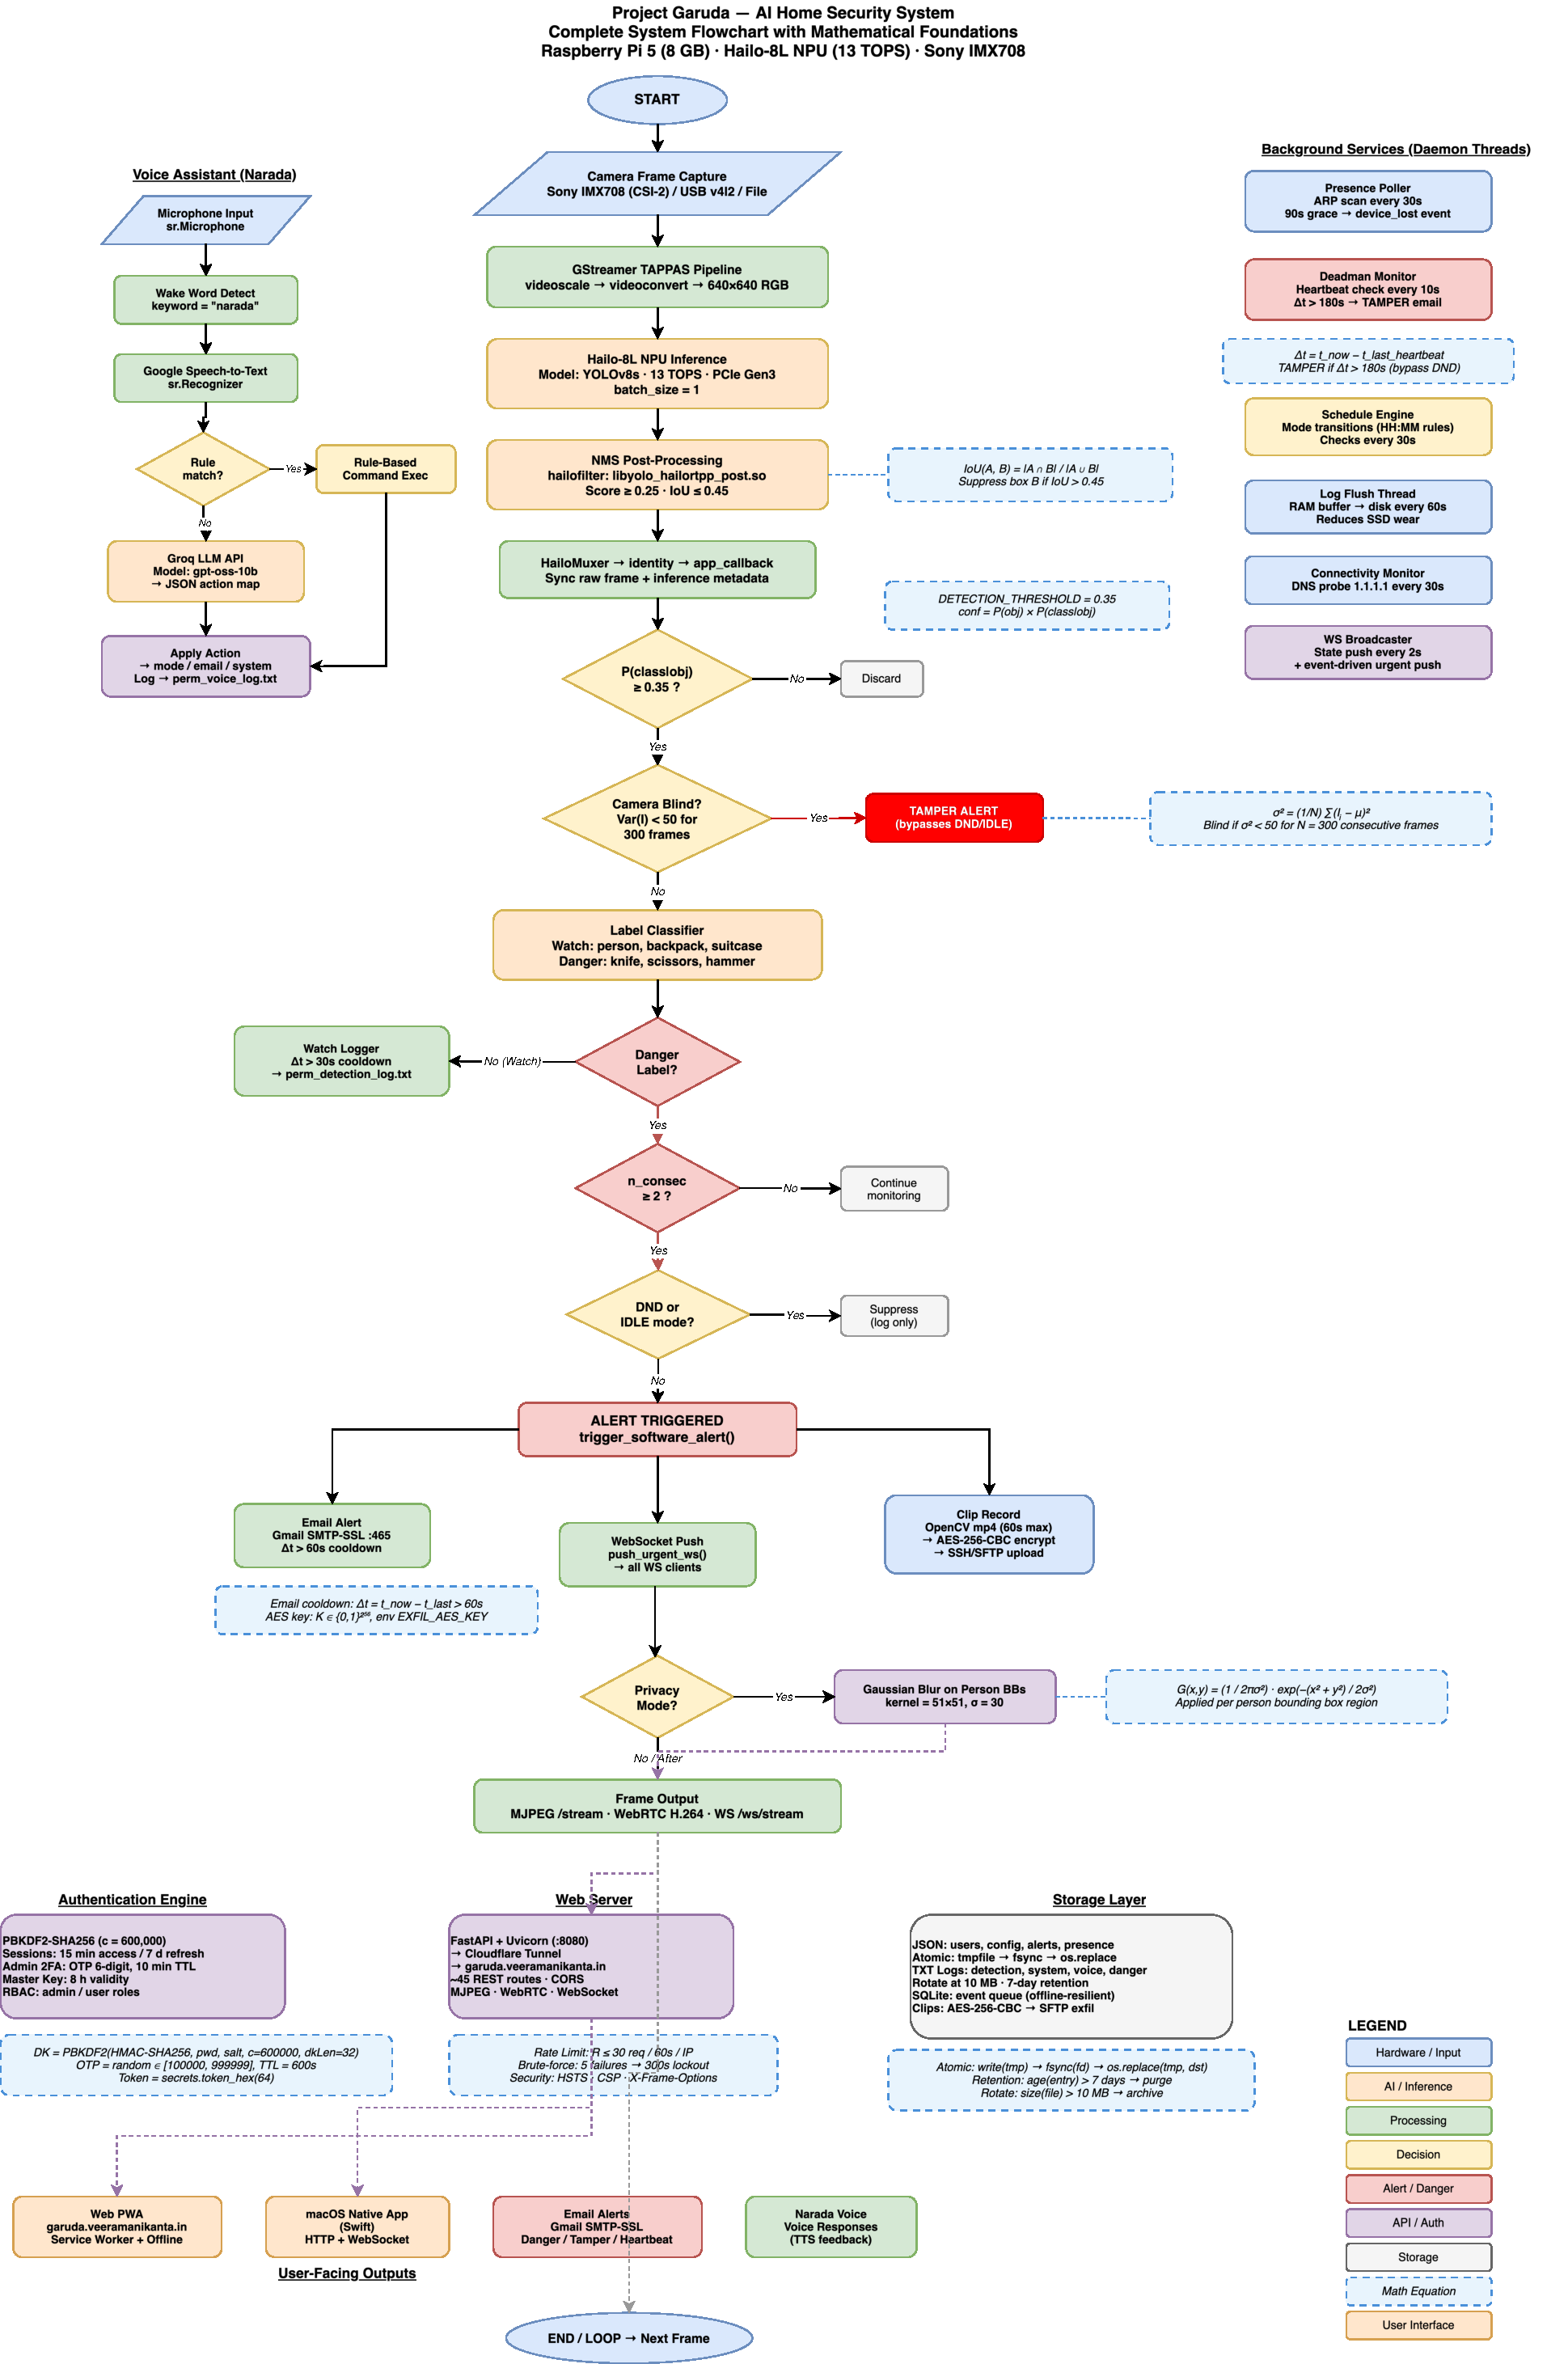
\includegraphics[width=\linewidth,height=0.72\textheight,keepaspectratio]{garuda_system_flowchart.drawio.pdf}
    \end{column}
  \end{columns}
\end{frame}

\begin{frame}{Models and Data}
  \begin{columns}[T]
    \begin{column}{0.56\textwidth}
      \begin{itemize}
        \item Primary detector: fine-tuned YOLOv8s for 4 classes.
        \item Classes: Person, Knife, Hammer, Scissors.
        \item Secondary verifier: MobileNetV2 on cropped detections.
        \item Extra pre-filter: MiDaS Small depth-variance cue for person-related screening.
      \end{itemize}
      \vspace{0.2cm}
      \begin{block}{Dataset snapshot}
        Final v5 corpus: 6,226 images, 5,311 annotated instances, 80/10/10 split.
      \end{block}
    \end{column}
    \begin{column}{0.44\textwidth}
      \centering
      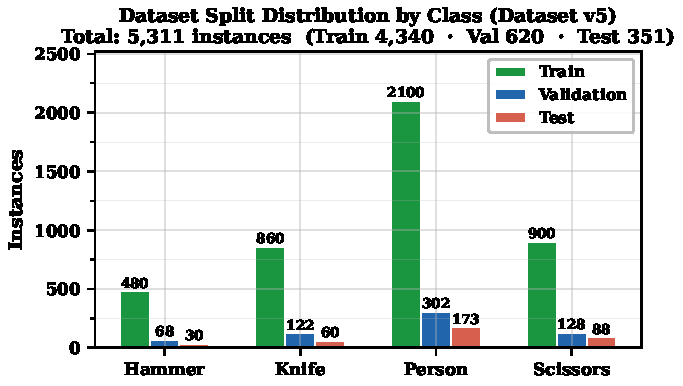
\includegraphics[width=\linewidth,height=0.64\textheight,keepaspectratio]{fig8_dataset_distribution.pdf}
    \end{column}
  \end{columns}
\end{frame}

\begin{frame}{Hardware and Deployment}
  \begin{columns}[T]
    \begin{column}{0.52\textwidth}
      \begin{itemize}
        \item Host: Raspberry Pi 5 with active cooling.
        \item Accelerator: Hailo-8L AI HAT+ (13 TOPS, INT8).
        \item Camera: Raspberry Pi Camera Module v3.
        \item Storage: SSD for models, logs, clips, and database.
      \end{itemize}
      \vspace{0.2cm}
      \begin{block}{Deployment principle}
        Neural inference uses the NPU; web, voice, alerting, and logging stay on the CPU side.
      \end{block}
    \end{column}
    \begin{column}{0.48\textwidth}
      \centering
      \includegraphics[width=\linewidth,height=0.68\textheight,keepaspectratio]{figures/fig_hardware_setup.pdf}
    \end{column}
  \end{columns}
\end{frame}

\begin{frame}{Key Detection Results}
  \begin{columns}[T]
    \begin{column}{0.52\textwidth}
      \begin{itemize}
        \item Test mAP@0.5 improved from 0.465 (v1) to 0.847 (v5).
        \item Overall test precision: 0.866.
        \item Overall test recall: 0.801.
        \item Best class: Scissors with mAP@0.5 of 0.967.
      \end{itemize}
      \vspace{0.2cm}
      \begin{block}{Interpretation}
        Performance gains mainly came from better dataset scale and diversity, not from changing the detector family.
      \end{block}
    \end{column}
    \begin{column}{0.48\textwidth}
      \centering
      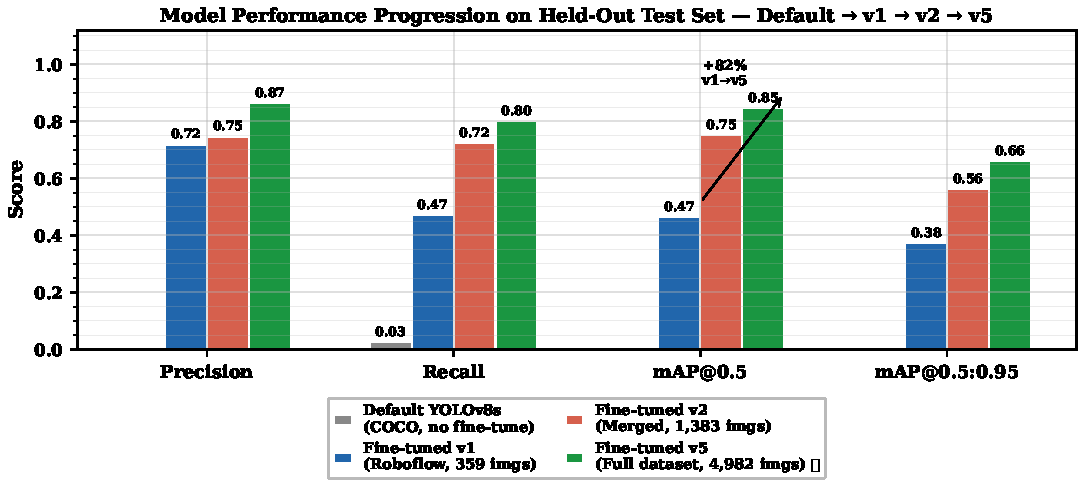
\includegraphics[width=\linewidth,height=0.68\textheight,keepaspectratio]{fig3_model_comparison.pdf}
    \end{column}
  \end{columns}
\end{frame}

\begin{frame}{Runtime Performance}
  \begin{columns}[T]
    \begin{column}{0.53\textwidth}
      \begin{itemize}
        \item On-chip throughput: 52.2 FPS.
        \item On-chip latency: 18.4 ms.
        \item Mean FPS across operating modes: $52.26 \pm 0.76$.
        \item Board power under load: $5.89 \pm 1.43$ W.
      \end{itemize}
      \vspace{0.2cm}
      \begin{block}{Why this matters}
        The pipeline stayed stable even while alerts, clip uploads, voice queries, and streaming were active.
      \end{block}
    \end{column}
    \begin{column}{0.47\textwidth}
      \centering
      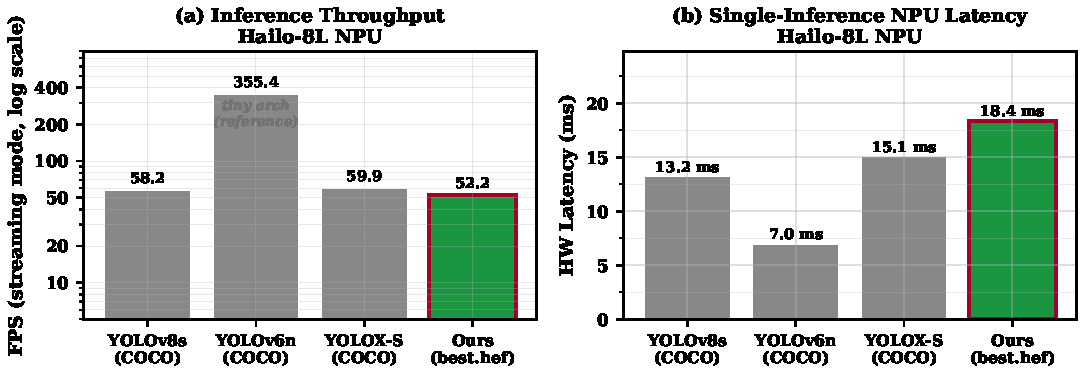
\includegraphics[width=\linewidth,height=0.32\textheight,keepaspectratio]{fig9_hardware_performance.pdf}
      
      \vspace{0.15cm}
      
\includegraphics[width=\linewidth,height=0.32\textheight,keepaspectratio]{fig13_fps_timeseries.pdf}
    \end{column}
  \end{columns}
\end{frame}

\begin{frame}{Privacy and Security Features}
  \begin{itemize}
    \item No image or video frames are sent to cloud inference services.
    \item Remote access is exposed through a Cloudflare tunnel instead of open port forwarding.
    \item Evidence clips are encrypted with AES-256-CBC before upload.
    \item Authentication uses PBKDF2-SHA256 with one-time-password support.
    \item Privacy mode can blur person detections before any on-LAN viewing path.
    \item Voice fallback sends short text only; raw audio and video remain local.
  \end{itemize}
\end{frame}

\begin{frame}{Main Takeaways}
  \begin{itemize}
    \item Garuda shows that a practical, privacy-first home-security stack can run fully at the edge on commodity hardware.
    \item The strongest contribution is system engineering: model integration, asynchronous design, and measured deployment behavior.
    \item The platform combines detection quality, real-time speed, and secure service integration without recurring cloud dependence.
  \end{itemize}
  \vspace{0.3cm}
  \begin{block}{Next steps}
    Longer real-world deployment studies, nuisance-condition testing, stronger anti-spoofing, and broader class coverage.
  \end{block}
\end{frame}

\begin{frame}
  \centering
  \Large Thank you
  
  \vspace{0.4cm}
  \normalsize Questions?
\end{frame}

\end{document}
